% Chapter: From Macro to Micro Architecture (blood pressure audit + hemodynamic attenuation).
% Standalone-compilable. To drop into the thesis, keep the body and merge the \bibitem entries.
% Figures are read from ../figures/ (in the thesis, set \graphicspath or prefix fig/).

\documentclass[11pt]{report}
\usepackage[margin=1.1in]{geometry}
\usepackage{amsmath,amssymb,booktabs,graphicx,microtype}
\usepackage[T1]{fontenc}
\usepackage[font=small,labelfont=bf]{caption}
\usepackage{xcolor}
\usepackage{hyperref}
\hypersetup{colorlinks=true,allcolors=blue!55!black}
\graphicspath{{../figures/}}

\newcommand{\kstar}{k^\star}
\newcommand{\Ltriv}{L_{\mathrm{triv}}}

\begin{document}
\setcounter{chapter}{4}
\chapter{From Macro to Micro Architecture}
\label{ch:micro}

%=========================================================================================
\section{Overview}

The circulation works at two scales. In the macrocirculation, the large arteries, each heartbeat
sends a pressure wave from the heart to the periphery, and the timing of that wave carries
information about blood pressure. In the microcirculation, small vessels match local supply to
local demand. In the brain this matching is tuned continuously. Astrocytes help raise flow where
neurons are active, collateral vessels take over when a route is lost, and vessels that carry
little flow are gradually pruned. This chapter draws on both scales. The physics of the large
arteries defines what a correct blood pressure model must compute, and the regulation of the
microcirculation suggests how a model should allocate its own computation.

Blood pressure is the motivating measurement. Wearable devices now stage sleep, estimate heart
rate from light passed through the skin, and remove motion noise as it happens, all continuously
on a device the size of a watch face. Blood pressure, one of the most basic hemodynamic
measurements, is still taken much as it was around 1900. A cuff is inflated around the upper arm
until it stops the flow of blood, then slowly released while the device listens for the sounds, or
senses the pressure oscillations, of blood forcing its way back through the compressed artery. The
result is a single reading of a quantity that changes with every heartbeat. The continuous
reference is a catheter with a pressure sensor placed inside an artery, used only in intensive care
and during surgery. Neither allows continuous monitoring in daily life.

Pulse transit time offers a way around both. Timing the pressure wave between two points on the
body gives its speed, and the wave travels faster when pressure is higher. The artery, however, is
not a passive pipe. When the left ventricle ejects blood into the aorta, the blood itself moves at
about 1~m/s at peak systole, while the stretch of the arterial wall travels along the arterial tree
at 4 to 15~m/s, depending on how stiff the arteries are. Transit time measures this wave in the
wall, and the stiffness of the wall depends on pressure in a way that differs between people
(Section~\ref{sec:bp_background}). A cuffless estimator can therefore match reference pressure on
a benchmark while computing nothing related to pulse propagation, and accuracy alone cannot reveal
this.

Chapter~3 constrained what a model sees and how it decides, restricting the inputs to
hemodynamic and motion sensors and reducing a gradient-boosted model to a cascade a person can
read. Chapter~4 used the macrocirculation to constrain the macro
architecture of a model, at the level of cross-attention between measurement sites. This chapter
moves inside the model. Project~3A (Section~\ref{sec:audit}) uses the physics of the large arteries
to verify a model: a mechanistic audit tests whether an estimator's prediction depends on transit
time in the way the physics requires, with preliminary results on a synthetic testbed. Project~3B
(Section~\ref{sec:3b}) uses the regulation of the microcirculation to build the model: a rule we
call hemodynamic attenuation closes attention heads during training, the way unneeded vessels
regress, until only the circuit the task needs remains, bringing a deep model closer to the
readability of the Chapter~3 cascade. The two meet in a joint experiment. A blood
pressure model trained with hemodynamic attenuation keeps only a few heads, and the audit of 3A can
then ask which of them, if any, carries transit time (Section~\ref{sec:joint}).

%=========================================================================================
\section{Background}
\label{sec:bp_background}

\subsection{Transit time and pressure}

The speed of a pressure wave in an elastic tube is given by the Moens--Korteweg relation,
$\mathrm{PWV} = \sqrt{E h / (\rho d)}$, where $E$ is the elastic modulus of the wall, $h$ its
thickness, $d$ the vessel diameter and $\rho$ the density of blood. The wall stiffens as pressure
rises, which is commonly modelled as $E = E_0 e^{\zeta P}$ \cite{hughes1979}. Combining the two gives
\begin{equation}
\mathrm{PWV} = \sqrt{\frac{E_0 h}{\rho d}}\; e^{\zeta P/2},
\qquad
P = \frac{2}{\zeta}\ln \mathrm{PWV} - \frac{1}{\zeta}\ln\frac{E_0 h}{\rho d}.
\label{eq:mk_bp}
\end{equation}
Pressure is a logarithmic function of wave speed with constants that differ between people, which
is why transit-time methods need calibration \cite{mukkamala2015}.

\subsection{Arrival time is not transit time}

Most cuffless systems measure pulse arrival time (PAT), from the R-peak of the ECG to the foot of
the pulse in a peripheral PPG. This interval also contains the pre-ejection period, the delay
between the electrical activation of the heart and the opening of the aortic valve:
\begin{equation}
\mathrm{PAT} = \mathrm{PEP} + \mathrm{PTT}.
\label{eq:pat}
\end{equation}
PEP changes with contractility and sympathetic tone independently of arterial pressure, so any
model trained on PAT inherits this confound. For a site at path length $d_i$ from the heart,
$\mathrm{PAT}_i = \mathrm{PEP} + d_i/\mathrm{PWV}$, so the difference between two sites cancels
PEP. Deep networks trained on raw ECG and PPG inherit the confound without showing it, and may also
use regression toward the population mean, demographic priors, or waveform shape unrelated to
propagation.

\subsection{Accuracy cannot certify mechanism}

% TODO: replace this paragraph with the formal statement of the non-identifiability result.
Two estimators with the same error on a dataset can compute different functions of their input.
One routes its prediction through transit time. The other routes it through confounds that happen
to vary with pressure in that dataset. The two diverge only under distribution shift, which is the
condition of deployment. Verifying a model therefore requires intervening on it, not only
evaluating its outputs.

%=========================================================================================
\section{Project 3A: A Mechanistic Audit for Blood Pressure Estimators}
\label{sec:audit}

The audit asks whether an estimator's prediction depends on transit time in the direction and
magnitude that Equation~\eqref{eq:mk_bp} requires. It has three tiers of increasing strength.
\begin{enumerate}
\item Linear probes test whether PTT can be read linearly from the model's internal activations.
\item Nonlinear probes test whether it can be read at all, separating absence from nonlinear
      encoding.
\item Causal tests intervene on the model. PTT-direction ablation removes the decoded direction and
      measures the change in prediction. Donor-swap activation patching transplants activations
      from an input with a different transit time and checks that the prediction moves by the
      amount the physics predicts. A roll test delays the distal PPG, which lengthens PTT, so the
      predicted pressure must fall. Each effect must have the correct sign and a physically
      plausible size.
\end{enumerate}
A model that is accurate but fails every tier is classified as not encoding transit time. At run
time such a model abstains rather than reporting a pressure it cannot justify.

\paragraph{Synthetic testbed.} Real data cannot validate an audit, because the true mechanism of a
trained network is unknown. We therefore built a testbed in which it is known. Part~1 is a scalar
task solved by three small networks with different, known mechanisms. Part~2 is a time-domain
tube-load waveform simulator in which foot-to-foot PTT was verified to be unchanged by the load
parameter $\Gamma$.
% CHECK: name what Gamma denotes in the simulator.

\paragraph{Preliminary result.} Across the Part~2 sweep, the donor-swap effect increased steadily
with $\alpha$, the degree to which the model relies on transit time, while accuracy stayed flat.
% TODO: confirm the definition of alpha and add the figure.
Accuracy did not change and the audit did, which is direct support for the argument that accuracy
cannot certify mechanism.

\paragraph{Remaining work.} Part~3 applies the audit to published architectures trained on real
ECG and PPG. Whether most such models fail the audit is the hypothesis of that experiment, not yet
a result. We also piloted a camera-based measurement of transit time between the face and the
hand. The remote PPG signals were too noisy to give reliable transit times, and camera-based
systems of this kind have already been reported \cite{jeong2016}, so this route is not pursued.

%=========================================================================================
\section{Project 3B: Hemodynamic Attenuation of the Micro Architecture}
\label{sec:3b}

An audit is only practical when the computation it examines is small. In the microcirculation,
supply is not fixed in advance. Vessels are kept where they are needed and pruned where they are
not. Project~3B applies the same idea to attention heads. In Chapter~4, a trained
transformer carried its causal computation in two of forty heads, but this was found only after
training, by ablating each head in turn, and the number of heads to keep had to be chosen by hand.
Project~3B asks whether a model can find the number of heads it needs during training, without
being given it. We introduce a rule for this, hemodynamic attenuation, and test it on tasks whose
minimal number of heads is known.

\subsection{Motivation from cerebral blood supply}

Four properties of cerebral blood supply motivate the rule:
\begin{enumerate}
\item Supply follows need. Local blood flow rises with neural activity, signalled in part by
      astrocytes \cite{attwell2010}. Each head is given a valve $g_h \in [0,1]$.
\item A vessel is dispensable when collateral vessels can supply its tissue \cite{faber2014}. A
      head is valued by what is lost when it closes and the other heads compensate, which we call
      its collateral value.
\item Maintaining a vessel has a metabolic cost \cite{murray1926}. Each open head has a fixed price,
      and there is no target number of heads.
\item Unneeded vessels regress gradually \cite{chen2012,franco2015}, and collaterals can enlarge
      when a route is blocked \cite{faber2014}. Closing heads fade out over 100 training steps and
      can be reopened.
\end{enumerate}
The biology motivates the design, and no claim is made about the brain.

\subsection{Astrocytes and attention}

Softmax attention turns a query's scores $s_1, \dots, s_N$ into weights
\begin{equation}
a_i = \frac{e^{s_i}}{\sum_j e^{s_j}} ,
\end{equation}
a numerator that differs for each memory slot and a denominator that is one number shared by all
of them. Kozachkov et al.\ \cite{kozachkov2023} showed that a network of neurons and one astrocyte
can approximately compute self-attention. The neurons store the numerators in Hebbian synapses.
The astrocyte computes the denominator. It pools activity across all the synapses it wraps and
scales every one of them by the same gain, $1/p_t$. For token $t$ the output is approximately
(their Eq.~11)
\begin{equation}
\ell_t \approx \frac{1}{p_t} \sum_i e^{k_i^{\top} q_t}\, v_i + x_t,
\qquad p_t = \sum_j e^{k_j^{\top} q_t},
\end{equation}
which is softmax attention plus a residual connection. The point used here is that the astrocyte
acts as a single gain on a whole block of synapses.

\subsection{Head pruning}

Michel et al.\ \cite{michel2019sixteen} remove heads by a gradient score, and Voita et al.\
\cite{voita2019analyzing} learn head gates with an $L_0$ penalty. Optimal Brain Damage \cite{obd}
scores a parameter by the loss increase when it is removed, and Optimal Brain Surgeon \cite{obs} by
the increase after the remaining parameters are re-fitted. ZipLM \cite{ziplm} applies the latter to
whole heads of trained language models. All of these prune after training, to a size chosen by the
user.

\subsection{Task}

\begin{figure}[t]
\centering
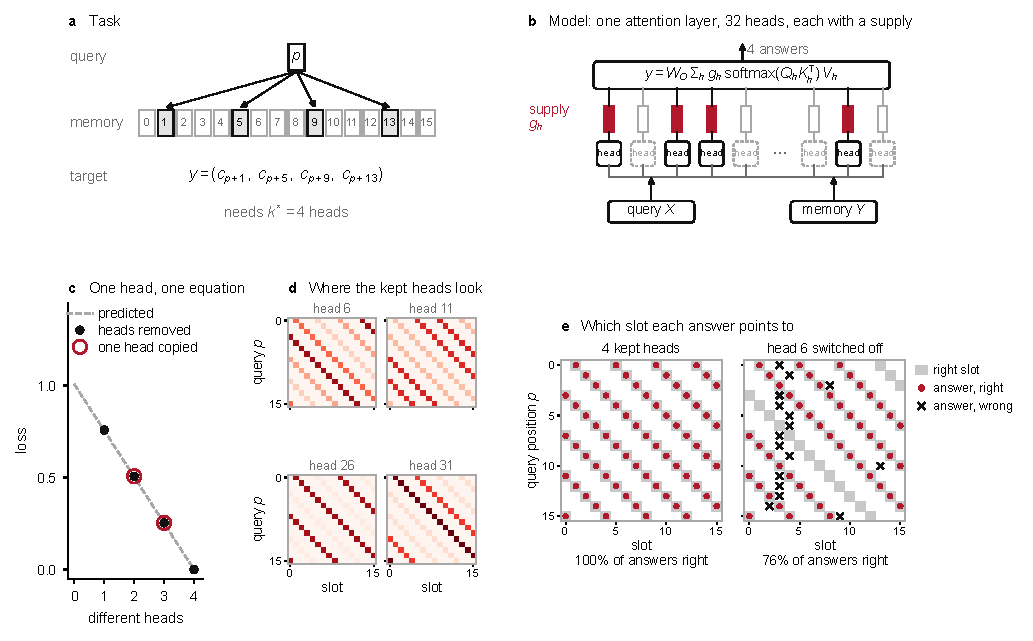
\includegraphics[width=\linewidth]{fig_setup.pdf}
\caption{Task and model.
\textbf{a}, A query carries a position $p$, and the target is the items stored $1, 5, 9, 13$ slots
ahead, so 4 heads are needed.
\textbf{b}, One attention layer with 32 heads, each with a valve $g_h$. Filled valves are open.
\textbf{c}, Loss with $k$ different heads on a trained 4-head model, against the prediction
$1 - k/4$.
\textbf{d}, The slot each answer points to. All are correct with the 4 kept heads, and 76\% with
head 6 switched off.}
\label{fig:setup}
\end{figure}

The memory has $N = 16$ slots, each holding a random item $c_j$. A query specifies a position $p$,
and the target is the items at $R$ fixed offsets (Figure~\ref{fig:setup}a):
\begin{equation}
\text{target}(p) = \big(c_{p+\delta_1},\ \dots,\ c_{p+\delta_R}\big),
\qquad \text{slots modulo } N.
\end{equation}
Items are redrawn for every example, so the model must learn where to attend.

A head returns, for each query, one weighted average of the items, which is one linear equation in
the $R$ unknown items. Recovering $R$ items needs $R$ independent equations, so the task needs
$\kstar = R$ heads, and with $k < R$ heads the lowest achievable loss is
\begin{equation}
\text{loss}(k) = \Big(1 - \frac{k}{R}\Big)\, \Ltriv,
\label{eq:law}
\end{equation}
where $\Ltriv$ is the loss of predicting the mean. Duplicate heads give the same equation and count
once. Measured losses agree with Equation~\eqref{eq:law} to within 1\% (Figure~\ref{fig:setup}c).
The task counts as solved when the loss is below $0.02\,\Ltriv$. Results are unchanged for any
threshold from $0.01$ to $0.1$.

\subsection{Model}

The model is one cross-attention layer with $H = 32$ heads and no MLP. Matrices have one column per
token, as in \cite{kozachkov2023}, with $X$ holding the queries and $Y$ the memory. Head $h$
computes the usual attention,
\begin{equation}
O_h = V_h\, \mathrm{softmax}\!\Big(\frac{K_h^{\top} Q_h}{\sqrt{d_k}}\Big),
\qquad Q_h = W_Q^h X,\quad K_h = W_K^h Y,\quad V_h = W_V^h Y,
\end{equation}
with the softmax taken down each column, so each query's weights over the memory add up to one.
Each head's output is multiplied by its valve $g_h$ before the heads are added together:
\begin{equation}
\hat{T} = \sum_{h=1}^{H} g_h\, W_O^h\, O_h .
\label{eq:valve}
\end{equation}
A head with $g_h = 0$ contributes nothing and receives no gradient, so a model with $k$ open valves
is exactly a $k$-head model. The valve plays the same algebraic role as the astrocyte gain, one
number that multiplies a whole block of synapses, here the output weights $W_O^h$ of one head. The
two differ in what sets them and how fast they change. The astrocyte gain follows pooled input
activity and changes with every token to normalise attention, while the valve follows the head's
collateral value and changes slowly over training to select heads. The correspondence is
algebraic only.

\subsection{Hemodynamic attenuation}
\label{sec:rule}

All valves start open. After a warm-up of 10\% of training, every 25 steps the rule (1) computes
the collateral value of every open head, (2) closes the lowest-valued head if its value is below the
price $0.03\,\Ltriv$, and (3) reopens the highest-valued closed head if its value exceeds twice the
price. A closing valve decreases by $1/100$ per step.

The collateral value is the increase in the best-fit loss when head $h$ is removed and the other
open heads re-fit their output weights:
\begin{equation}
v_h = \min_W L(\text{without } h) - \min_W L(\text{all open heads}).
\end{equation}
This is the Optimal Brain Surgeon score \cite{obs}, applied to whole heads as in ZipLM
\cite{ziplm}, and it is computed in closed form from one matrix inverse. The score is not new. The
contribution is its use during training, with a price, a gradual fade, and reopening. The re-fit
is what makes a copy worthless. If two heads output the same signal with weights $(0.5, 0.5)$,
removing one without re-fitting halves the output, so both look important. With re-fitting the
other head takes weight 1, the loss does not change, and the copy is worth nothing.

\subsection{Baselines and evaluation}

All methods share the model, task, training and runs. The published methods are run inside our
training: ZipLM-style pruning \cite{ziplm} (the same score applied once, then fine-tuning), Michel
et al.\ \cite{michel2019sixteen}, and Voita et al.\ \cite{voita2019analyzing}. Three controls each
remove one part of the rule: no fade, no re-fit (the Optimal Brain Damage score \cite{obd}), and no
score (random choice). We report exact count (open heads over the last 40\% of training equal
$\kstar$) and never broke (after first falling below the solved threshold, the loss never exceeds
it), on $\kstar = 2, 4, 8$ with 10 seeds each, together with runs with duplicated heads, runs with
random head failure, and a two-layer induction task \cite{olsson2022}.

\subsection{Preliminary results}

\begin{figure}[t]
\centering
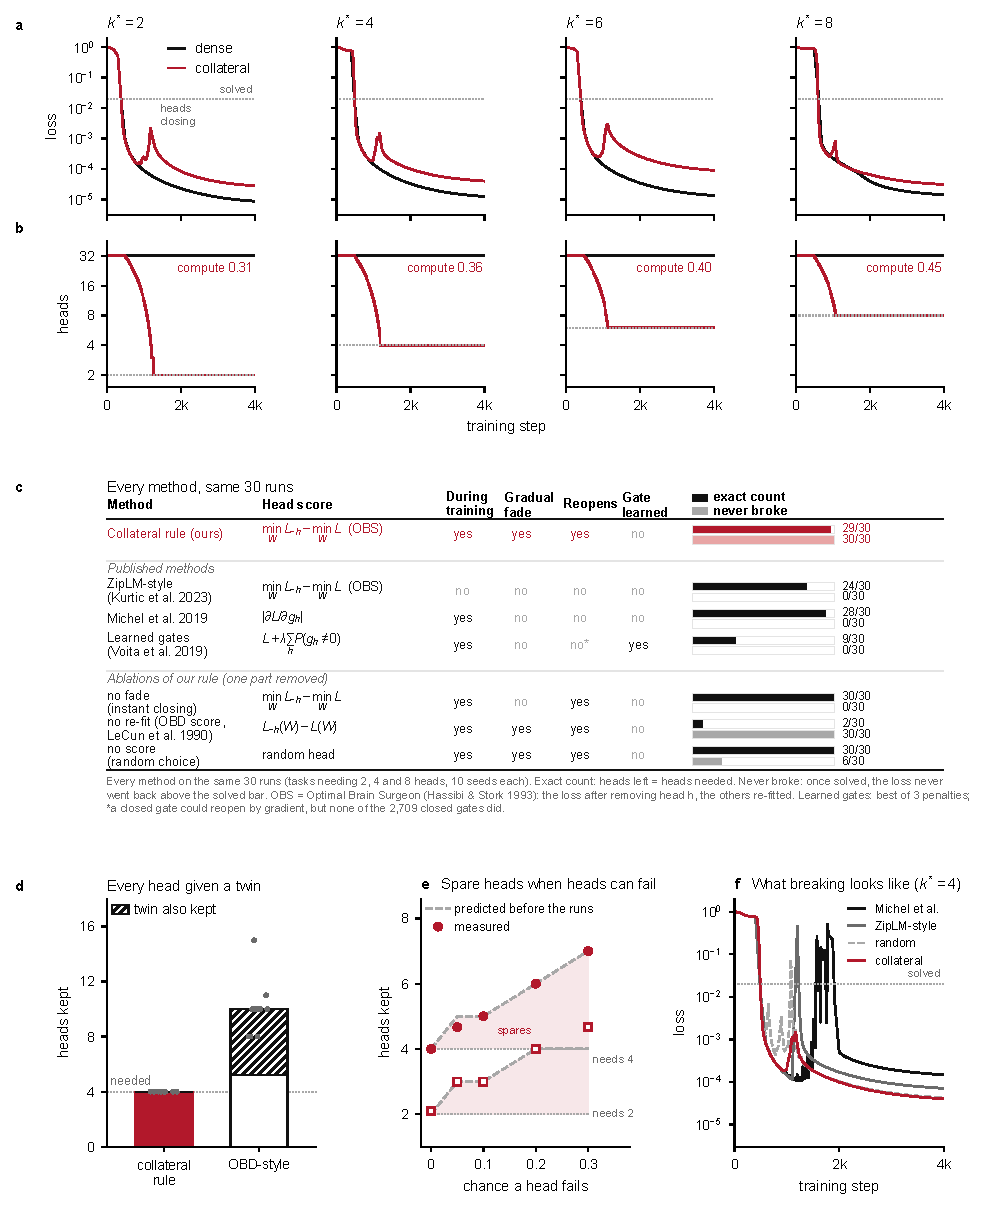
\includegraphics[width=\linewidth]{fig_main.pdf}
\caption{Hemodynamic attenuation during training.
\textbf{a}, Loss of the dense model (black) and with hemodynamic attenuation (red).
\textbf{b}, Open heads, with $\kstar$ dotted.
\textbf{c}, All methods on the same 30 runs.
\textbf{d}, Runs in which every head starts with an identical copy.
\textbf{e}, Spare heads kept under random failure, against the prediction.
\textbf{f}, One run per method. Only hemodynamic attenuation stays below the solved threshold.}
\label{fig:main}
\end{figure}

\paragraph{Count and stability.} Hemodynamic attenuation kept exactly $\kstar$ heads in 29 of 30
runs and never broke the model in 30 of 30. No other method achieved both
(Figure~\ref{fig:main}c). Without the fade the model broke in every run. Without the re-fit it kept
too many heads. With random choice it broke in 24 of 30 runs.

\paragraph{Duplicated heads.} With every head starting as a copy of another, the rule kept 4 heads
and never both members of a pair. Without the re-fit, 8 to 15 heads and 4 to 7 pairs were kept
(Figure~\ref{fig:main}d).

\paragraph{Backup heads.} When heads fail at random, the rule should keep extra heads in proportion
to how likely they are to be needed. A formula written before the experiments predicted the number
kept exactly in 21 of 24 runs and to within one head in the rest (Figure~\ref{fig:main}e).

\paragraph{Induction.} In a two-layer attention-only model with 8 + 8 heads, the minimal induction
circuit is one previous-token head and one induction head \cite{olsson2022}. Hemodynamic attenuation
kept 2 + 1 heads in 10 of 10 runs and never broke the model. The kept heads had the expected roles
in all 10 runs, and switching off the induction head reduced next-token accuracy on the repeat to
zero (Figure~\ref{fig:induction}). Layer 2 reached the needed single head, while layer 1 kept two.
Every method kept the same 2 + 1 heads on this task, so only stability separated them. The method
of Michel et al.\ broke the model in all 10 runs.

\begin{figure}[t]
\centering
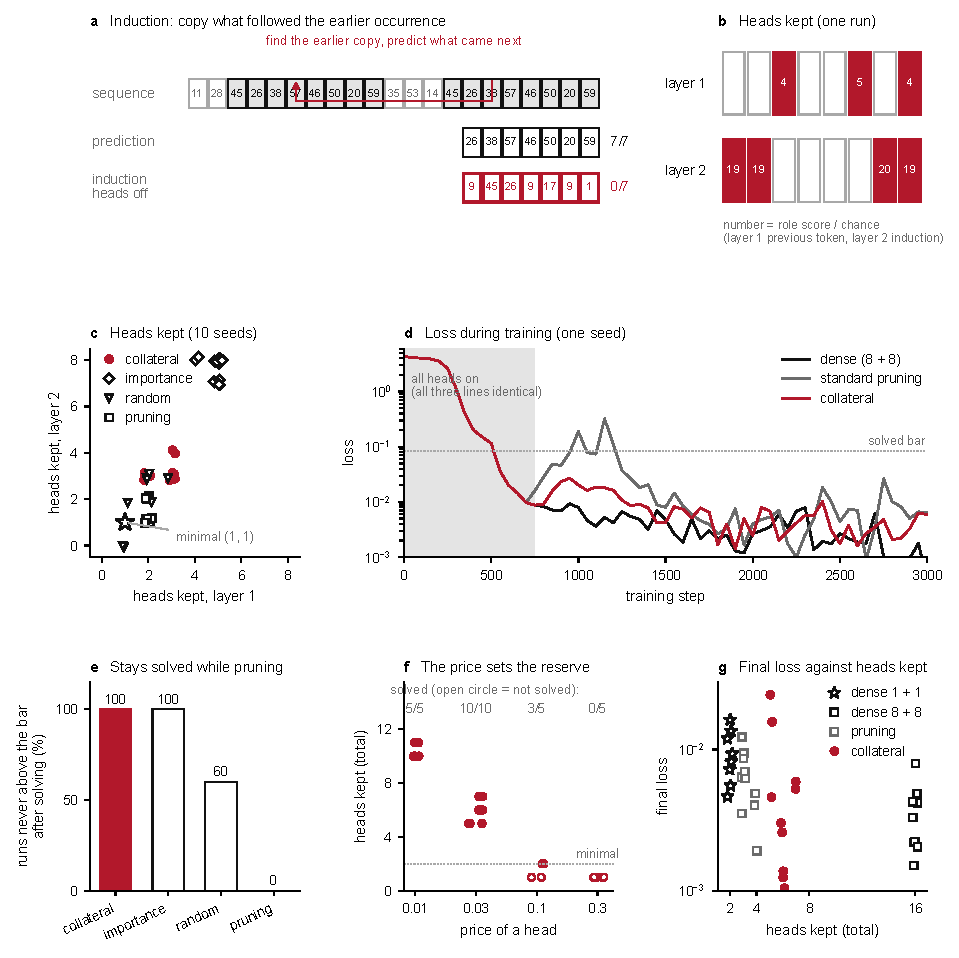
\includegraphics[width=\linewidth]{fig_induction.pdf}
\caption{Two-layer induction.
\textbf{a}, An example sequence and the model's predictions on the repeat, with all kept heads
(7/7 correct) and with the layer-2 head switched off (0/7).
\textbf{b}, Attention of the kept heads on that sequence. The layer-1 head looks one token back, and
the layer-2 head looks at the token after the earlier copy.
\textbf{c}, Open heads in each layer during training, 10 runs. Layer 2 reaches the needed one head,
and layer 1 stops at two.
\textbf{d}, Runs that never broke, 10 per method, all with the same settings.
\textbf{e}, Loss during training for one seed.}
\label{fig:induction}
\end{figure}

\paragraph{Cost.} The final loss was 2 to 7 times the dense model's, well below the threshold, using
0.31 to 0.45 of its head-steps. The saving is nominal, since closed heads are still computed.

\subsection{Joint experiment: attenuate, then audit}
\label{sec:joint}

The two projects meet in one experiment. A transformer is trained to estimate blood pressure on
the synthetic tube-load testbed of Project~3A, where the role of transit time is known, with
hemodynamic attenuation closing heads during training. The audit of Project~3A is then run on each
of the few heads that remain. If the model computes pressure from transit time, the audit should
find it in a small number of named heads, and switching those heads off should move the predicted
pressure in the direction the physics requires. If no surviving head carries transit time, the
model is accurate for another reason, and the audit has caught it with far fewer heads to check.

\subsection{Proposed work}

The proposed work follows the timeline in Figure~\ref{fig:timeline}. It begins with the joint
experiment of Section~\ref{sec:joint}, which trains a blood pressure model with hemodynamic
attenuation and audits the heads that remain.

The rule currently values a head by re-fitting only the final read-out. Between layers, one layer's
heads change what the next layer attends to, and a re-fit at the output cannot repair that. This is
why layer 1 of the induction model keeps one head more than needed. The proposed extension values a
head at its own layer, by asking the other heads of that layer to rebuild what the next layer reads,
the same layer-wise approach used to prune large language models \cite{ziplm}. It will be developed
on small language models trained from scratch, where accuracy can be measured against the number of
open heads, and checked on the induction task, where it should reach the needed 1 + 1 heads.

The rule will then be applied to the models of Chapter~4, asking whether it keeps the two causal
heads found in qSA-Cross, and whether the same heads are kept across all sixteen
leave-one-subject-out folds of the Cross-Site Transformer on WildPPG. Finally, it will be applied
while fine-tuning GPT-2 small on indirect object identification, a task whose circuit in that model
is known \cite{wang2023}, asking whether the heads the rule keeps overlap with that circuit.

%=========================================================================================
\section{Timeline}

\begin{figure}[htbp]
\centering
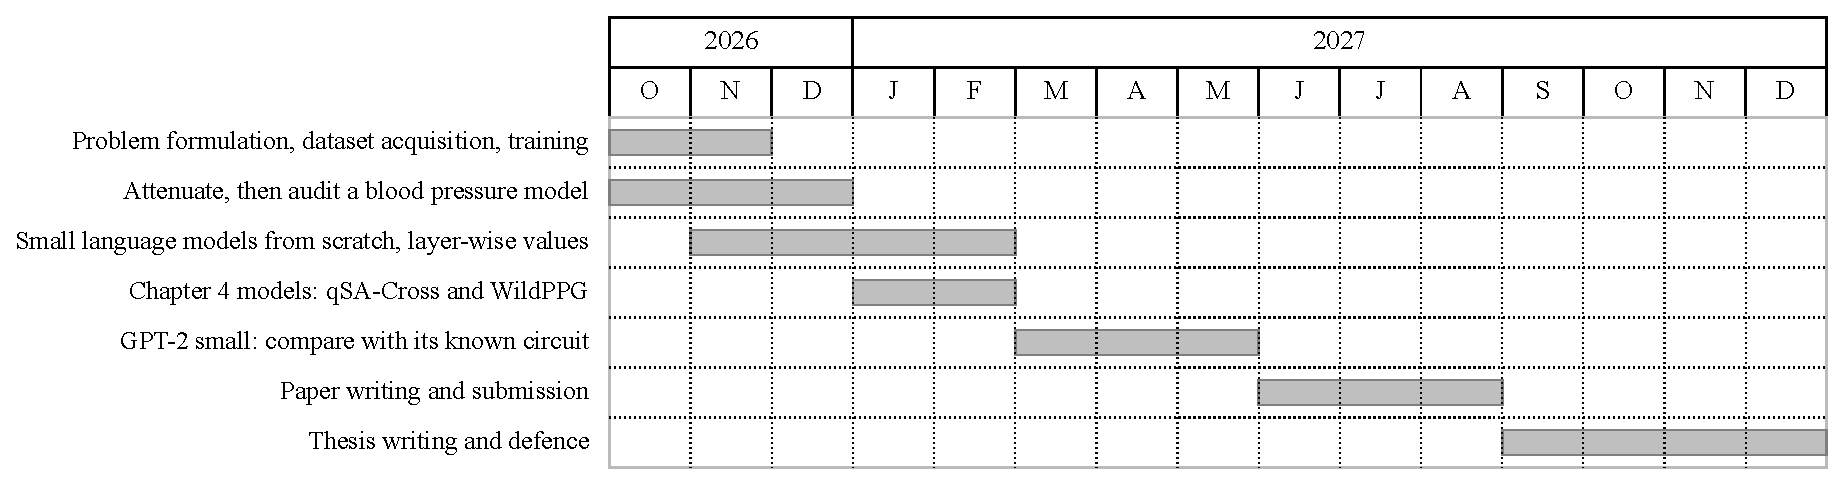
\includegraphics[width=\textwidth]{gantt_hmha.pdf}
\caption{Timeline from the proposal to the defence.}
\label{fig:timeline}
\end{figure}

%=========================================================================================
\section{Risks and Fallbacks}

\paragraph{The audit is inconclusive on real data.} The audit's contribution does not depend on new
human data. If published models cannot be retrained or their activations are unavailable, the audit
is reported on the synthetic testbed and on models trained here on public multi-site recordings.

\paragraph{The rule does not reach the minimum in deeper models.} This is already visible in the
induction task, where layer 1 keeps one extra head. If the layer-wise value does not close the gap,
the result is still a small circuit found during training, and the gap is reported with the number
of extra heads per layer.

\paragraph{The rule does not scale.} The collateral value needs one matrix inverse per layer. If this
is too costly for large models, it will be computed on a subset of layers or with the approximations
used in large-model pruning, and the accuracy of the approximation will be measured on the small
tasks where the exact value is known.

\paragraph{The kept heads differ from those found in Chapter~4.} This would be a finding about how
stable circuits are across training methods, and will be reported as such.

%=========================================================================================
\begin{thebibliography}{99}
% Check volume and page details against the originals before submission.
\bibitem{hughes1979} D.~J.~Hughes, C.~F.~Babbs, L.~A.~Geddes, J.~D.~Bourland. Measurements of
  Young's modulus of elasticity of the canine aorta with ultrasound. \emph{Ultrasonic Imaging}
  1(4):356--367, 1979.
\bibitem{mukkamala2015} R.~Mukkamala et al. Toward ubiquitous blood pressure monitoring via pulse
  transit time: theory and practice. \emph{IEEE Trans.\ Biomed.\ Eng.} 62(8):1879--1901, 2015.
\bibitem{jeong2016} I.~C.~Jeong, J.~Finkelstein. Introducing contactless blood pressure assessment
  using a high speed video camera. \emph{J.\ Med.\ Syst.} 40:77, 2016.
\bibitem{kozachkov2023} L.~Kozachkov, K.~V.~Kastanenka, D.~Krotov. Building transformers from
  neurons and astrocytes. \emph{PNAS} 120(34):e2219150120, 2023.
\bibitem{attwell2010} D.~Attwell, A.~M.~Buchan, S.~Charpak, M.~Lauritzen, B.~A.~MacVicar,
  E.~A.~Newman. Glial and neuronal control of brain blood flow. \emph{Nature} 468:232--243, 2010.
\bibitem{faber2014} J.~E.~Faber, W.~M.~Chilian, E.~Deindl, N.~van Royen, M.~Simons. A brief
  etymology of the collateral circulation. \emph{Arterioscler.\ Thromb.\ Vasc.\ Biol.}
  34(9):1854--1859, 2014.
\bibitem{murray1926} C.~D.~Murray. The physiological principle of minimum work: I.\ The vascular
  system and the cost of blood volume. \emph{PNAS} 12(3):207--214, 1926.
\bibitem{chen2012} Q.~Chen et al. Haemodynamics-driven developmental pruning of brain
  vasculature in zebrafish. \emph{PLoS Biol.} 10(8):e1001374, 2012.
\bibitem{franco2015} C.~A.~Franco et al. Dynamic endothelial cell rearrangements drive
  developmental vessel regression. \emph{PLoS Biol.} 13(4):e1002125, 2015.
\bibitem{obd} Y.~LeCun, J.~S.~Denker, S.~A.~Solla. Optimal brain damage. \emph{NeurIPS} 2, 1989.
\bibitem{obs} B.~Hassibi, D.~G.~Stork, G.~J.~Wolff. Optimal brain surgeon and general network
  pruning. \emph{IEEE International Conference on Neural Networks}, 1993.
\bibitem{ziplm} E.~Kurtic, E.~Frantar, D.~Alistarh. ZipLM: Inference-aware structured pruning
  of language models. \emph{NeurIPS}, 2023.
\bibitem{michel2019sixteen} P.~Michel, O.~Levy, G.~Neubig. Are sixteen heads really better than
  one? \emph{NeurIPS}, 2019.
\bibitem{voita2019analyzing} E.~Voita, D.~Talbot, F.~Moiseev, R.~Sennrich, I.~Titov. Analyzing
  multi-head self-attention: specialized heads do the heavy lifting, the rest can be pruned.
  \emph{ACL}, 2019.
\bibitem{olsson2022} C.~Olsson et al. In-context learning and induction heads.
  \emph{Transformer Circuits Thread}, 2022.
\bibitem{wang2023} K.~Wang, A.~Variengien, A.~Conmy, B.~Shlegeris, J.~Steinhardt. Interpretability
  in the wild: a circuit for indirect object identification in GPT-2 small. \emph{ICLR}, 2023.
\end{thebibliography}

\end{document}
